\subsubsection{Robotetik}
	Når der snakkes om selvkørende biler, bliver der ofte stillet etiske spørgsmål. Når man overfører kontrollen over bilen fra mennesket og overgiver dette til bilen selv, overføres også et stort ansvar. I tilfælde af at bilen kommer ud for et uheld, hvad skal bilen så gøre? Der er mange muligheder, men de kan ligeledes alle have store konsekvenser. Hvis en person ender foran bilen, skal den kunne træffe en beslutning om at forsøge at undvige personen og køre galt, eller om den blot skal forsøge at bremse. Hvis bilen bremser, er det ikke sikkert, at bilen kan nå at bremse for personen. Men hvis den forsøger at undvige, er det muligt, at den kører ind i med en modkørende bil. 

	Alt efter bilens programmering ville den kunne forsøge at minimere skader, ved at træffe det valg der vil forårsage færrest menneskeskader. Men dette kunne bringe uskyldige mennesker i fare, hvis bilen valgte at undvige en person ved at køre over i den anden side af vejen, hvor en modkørende bil kunne befinde sig. 
	
	Dette er et spørgsmål, som endnu ikke er besvaret fra de selvkørende biler, da dagens biler i en sådan situation vil overlade styringen til føreren. 

	En undersøgelse (se figur \ref{fig:etik_accident}) blev i 2014 foretaget af Open Roboethics Initiative, hvor mennesker blev adspurgt, om hvordan de ønskede at bilen skulle opføre sig i en situation som nævnt ovenfor. 52\% af de adspurgte mennesker ønsker, at bilen skal forsøge at minimere skaderne ved at fordele disse mellem både passagerer og fodgængere. 
	

	\begin{figure}[h!]
		\centering
		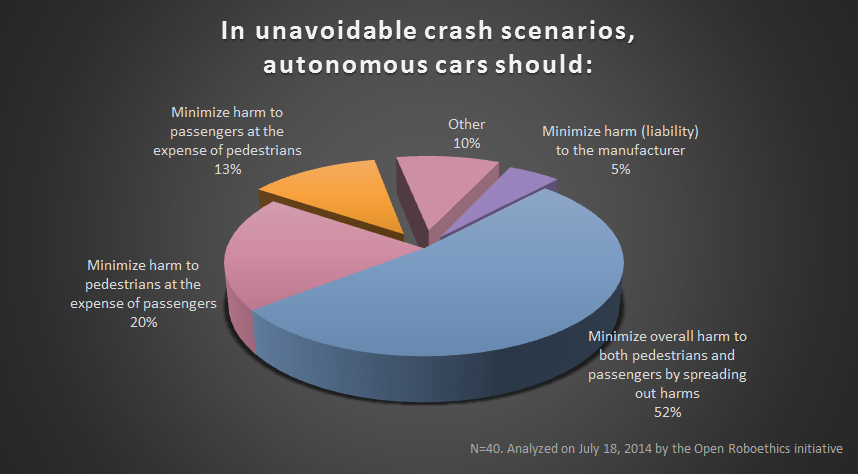
\includegraphics[width=\textwidth]{images/roboethics-2.jpg}
		\captionsource{Undersøgelse om hvad folk vil foretrække i en uundgåelig ulykke.}{\url{http://www.openroboethics.org/results-random-chance-over-informed-decision/}}
		\label{fig:etik_accident}
	\end{figure}

	I et scenarium, hvor et tog kommer kørende ned ad en bane imod tre mennesker spændt fast til togskinnerne, men inden toget støder mod disse tre personer, er der et baneskift. Hvis der på den anden række togskinner kun ligger \'en person, vil den logiske løsning være at skifte bane for toget, da der dermed reddes 2 menneskeliv. Men hvad hvis denne ene person er meget betydningsfuld for en, så som en mor eller ens egen søn, ville samme person så træffe samme valg og vælge at slå sit eget barn ihjel, frem for tre fremmede mennesker? En maskine vil stadig tænke logisk og træffe samme valg da færre liv går tabt, men ingen forældre vil have det komfortabelt med at benytte en bil, som kan træffe selv samme beslutning og slå deres eget barn ihjel, som muligvis sidder på bagsædet, frem for at ramme nogle fremmede fodgængere.
	
	Tilbage i 1942, præsenterede science fiction forfatteren Isaac Asimov, 3 gyldne love\cite{Asimov}, som siden er blevet brugt utallige gange til at beskrive, hvordan en robot hovedsageligt skal omgås mennesker.
	
	\begin{enumerate}
		
		\item En robot må ikke gøre et menneske fortræd, eller, ved ikke at gøre noget, lade et menneske komme til skade
		\item En robot skal adlyde ordrer givet af mennesker, så længe disse ikke er i konflikt med første lov
		\item En robot skal beskytte sin egen eksistens, så længe dette ikke er i konflikt med første eller anden lov
		
	\end{enumerate}
	
	Disse tre love er i bund og grund også etiske, da de siger at robotten ikke må adlyde et menneskes ordre, hvis dette forårsager skader på andre mennesker, men samtidig skal sørge for at mennesker ikke kommer til skade. Hvis et deprimeret individ springer ud foran en selvkørende bil i et forsøg på at begå selvmord, må bilen ikke bare køre personen over, da dette er i strid mod første lov. Bilen bliver derfor nødt til at undvige, også selvom dette kan totalskade bilen, og brække et legeme eller to på passageren, da et brækket ben er langt bedre end et mistet liv, samtidig med at overholde Asimov's 3 love. Her bliver føreren af bilen dog ``straffet'' for, at et andet menneske forsøger at tage sit eget liv. Skal bilen i dette tilfælde gøre det samme som føreren af en manuelt-kørende bil og køre ham ned da det er umuligt at undvige, selvom dette vil være i strid mod første lov? 

	Det kan være svært, at svare på disse spørgsmål og i sidste ende vil sådan nogle problemstillinger besvares, ved at politikere fastsætter love der giver producenterne nogle klare linjer at programmere efter.